\documentclass[hyperref, UTF8]{ctexart}
\usepackage{graphicx}
\usepackage{float}
\usepackage{amsmath}
\usepackage{amsfonts}
\usepackage{amssymb}
\usepackage{fontspec}
\usepackage{tikz}
\usepackage{booktabs}
\setmonofont{Consolas}
\setCJKmainfont{Noto Sans SC Regular}
\usetikzlibrary{shapes.geometric, arrows}
\tikzstyle{startstop} = [rectangle, rounded corners, minimum width=3cm, minimum height=1cm,text centered, draw=black, fill=red!30]
\tikzstyle{io} = [trapezium, trapezium left angle=70, trapezium right angle=110, minimum width=3cm, minimum height=1cm, text centered, draw=black, fill=blue!30]
\tikzstyle{process} = [rectangle, minimum width=3cm, minimum height=1cm, text centered, draw=black, fill=orange!30]
\tikzstyle{empty_process} = [rectangle, minimum width=3cm, minimum height=1cm, text centered, draw=none, fill=none]
\tikzstyle{decision} = [diamond, minimum width=3cm, minimum height=1cm, text centered, draw=black, fill=green!30]
\tikzstyle{arrow} = [thick,->,>=stealth]
\usepackage[a4paper, top=3cm, bottom=3cm, left=3cm, right=3cm]{geometry}
\usepackage{subcaption}
\usepackage{xcolor}
\usepackage{animate}
\usepackage{listings}
\lstset{
	keywordstyle=\color{blue!70},
	commentstyle=\color{red!50!green!50!blue!50},
	frame=shadowbox,
	rulesepcolor=\color{red!20!green!20!blue!20},
	tabsize=2,
	basicstyle=\ttfamily\small,
	numberstyle=\tiny,
	numbers=left,
	showstringspaces=false,
	breaklines=true,
	language=MATLAB
}
\hypersetup{
	colorlinks=true,
	bookmarks=true,
	bookmarksopen=true,
	pdftitle=遥感综合实验~遥感图像分类实验报告,
	pdfauthor=16020710017~蓝彧文,
	linkcolor=blue
}
\title{遥感综合实验实验报告\\遥感图像分类}
\author{蓝彧文~16020710017}
\begin{document}
	\maketitle
	\tableofcontents
	\newpage
	实验中使用的所有代码和数据可以在\\ \url{https://github.com/EwenLan/remote-sensing-library}获取。
	\section{实验四~无监督分类}
	\subsection{实验目的}
理解遥感图像分类的概念,掌握一些典型的图像无监督分类方法,例如K均值聚类算法。完成遥感图像的图像分类。
\subsection{实验原理}
\begin{figure}[H]
	\centering
	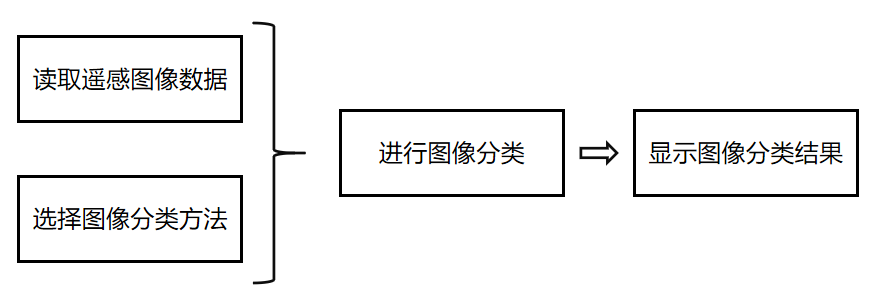
\includegraphics[width=0.7\linewidth]{figure/classification_flowchart.png}
	\caption{进行图像分类的步骤}
\end{figure}
\subsubsection{图像分类的概念}
将图像中的像素点划分为不同的类别,每一个类别具有特定的物理含义。例如不同的地物类型,包括草地、水泥地、建筑、道路、森林、山地等。

图像分类的两个步骤:特征提取和分类算法。
\begin{description}
	\item[特征提取] 如何描述每一个像素点,颜色特征向量。
	\item[分类算法] k均值据类算法。
\end{description}
\subsubsection{k均值聚类算法}
k均值据类算法是一个迭代算法,迭代更新每一个类别的聚类中心,并且通过最近邻准则完成分类。
\begin{description}
	\item[算法描述] \begin{enumerate}
		\item 任选K个初始聚类中心:$Z_1(1)$,$Z_2(1)$,$\dots$,$Z_K(1)$
		\item 按最小距离原则叫其余样本分配到K各聚类中心中的某一个,即
		\[ \text{若} \min\left\lbrace \left\| \mathbf{X}-\mathbf{Z}_i(k) \right\|,i=1,2,\dots,K \right\rbrace=\left\| \mathbf{X}-\mathbf{Z}_j(k) \right\|=D_j(k) \]
		则$X\in S_j(k)$
		\item  计算各个聚类中心的新向量值:$\mathbf{Z}_j(k+1)\quad j=1,2,\dots,K$
		\[ \mathbf{Z}_j(k+1)=\frac{1}{N_j}\sum_{\mathbf{X}\in S_j(k)}\mathbf{X}\quad j=1,2,\dots,K \]
		\item 如果$\mathbf{Z}_j(k+1)\neq\mathbf{Z}_j(k)\quad j=1,2,\dots,K$,则回到2,将模式样本逐个重新分类,重复迭代计算。
		\item 如果$\mathbf{Z}_j(k+1)=\mathbf{Z}_j(k)\quad j=1,2,\dots,K$,算法收敛,计算完毕。
	\end{enumerate} 
\end{description}
\subsection{实验流程}
\begin{figure}[H]
	\centering
	\begin{tikzpicture}[node distance=1.5cm]
	\node(start) [startstop] {开始};
	\node(input_img) [io, below of=start] {输入待分类的图像};
	\node(random_center) [process, below of=input_img] {随机选取聚类中心};
	\node(calculate_distance) [process, below of=random_center] {计算所有像素到每一个聚类点的距离};
	\node(classifing) [process, below of=calculate_distance] {根据距离对像素点归类};
	\node(convergent) [decision, below of=classifing, yshift=-1.5cm] {算法是否收敛?};
	\node(calculate_center) [process, right of=convergent, xshift=3cm] {重新计算聚类点的坐标};
	\node(display) [io, below of=convergent, yshift=-1.5cm] {显示聚类结果};
	\node(end) [startstop, below of=display] {结束};
	
	\draw[arrow] (start) -- (input_img);
	\draw[arrow] (input_img) -- (random_center);
	\draw[arrow] (random_center) -- (calculate_distance);
	\draw[arrow] (calculate_distance) -- (classifing);
	\draw[arrow] (classifing) -- (convergent);
	\draw[arrow] (convergent) -- node[anchor=east] {是} (display);
	\draw[arrow] (convergent) -- node[anchor=south] {否} (calculate_center);
	\draw[arrow] (calculate_center) |- (calculate_distance);
	\draw[arrow] (display) -- (end);
	\end{tikzpicture}
\end{figure}
\subsection{实验程序}
\lstinputlisting[caption={K均值聚类程序}]{"../Executable Script/Exp 4/ReadAirportImages.m"}
\subsection{实验结果和分析}
对如图\ref{fig:airport_44}所示的图片上的像素进行聚类。设置聚类数为$2$,初始聚类中心设置为随机数,可以得到如图\ref{fig:airport_44_class_1_logical}和图\ref{fig:airport_44_class_2_logical}所示的分类结果。
\begin{figure}[H]
	\centering
	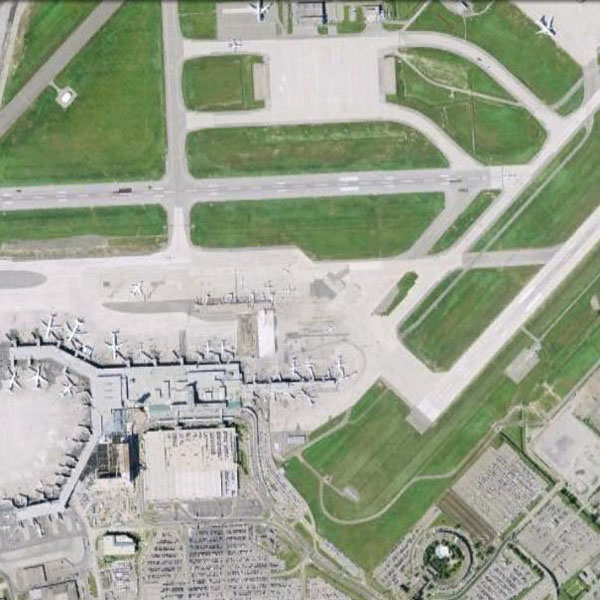
\includegraphics[width=0.7\linewidth]{figure/airport_44.jpg}
	\caption{飞机场原图}
	\label{fig:airport_44}
\end{figure}
\begin{figure}[H]
	\centering
	\begin{minipage}{0.45\linewidth}
		\centering
		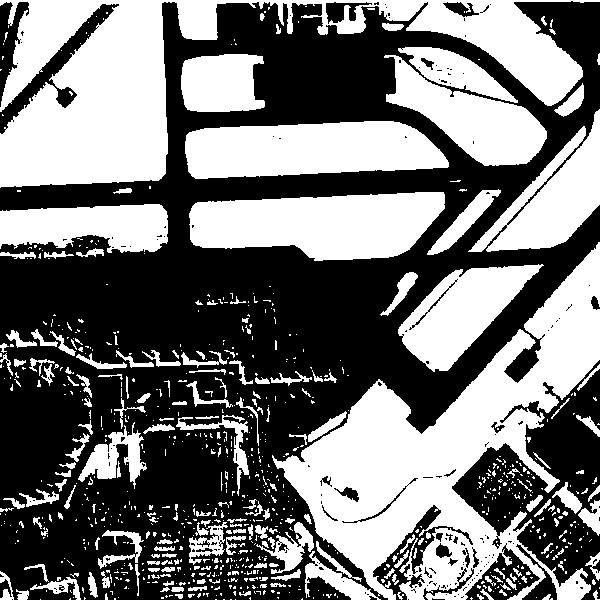
\includegraphics[width=\linewidth]{figure/airport_44_Class_01_Logical.png}
		\caption{第一个分类的分类图}
		\label{fig:airport_44_class_1_logical}
	\end{minipage}
	\begin{minipage}{0.45\linewidth}
		\centering
		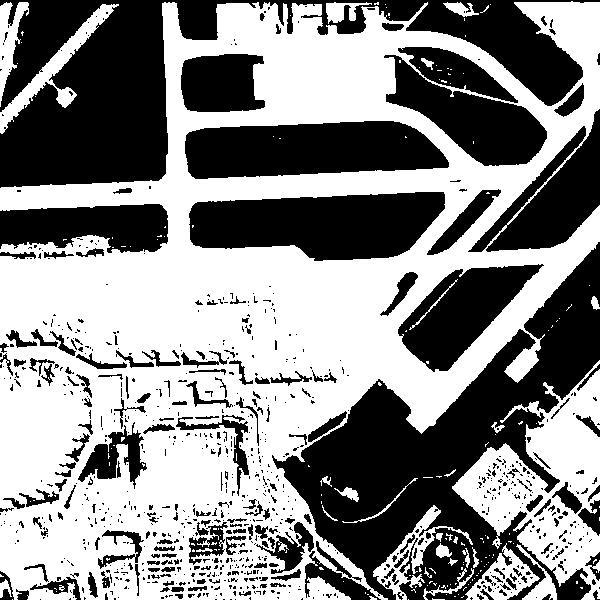
\includegraphics[width=\linewidth]{figure/airport_44_Class_02_Logical.png}
		\caption{第二个分类的分类图}
		\label{fig:airport_44_class_2_logical}
	\end{minipage}
\end{figure}
其中,逻辑分类图中的白色区域代表图片中这个区域的像素点属于这一个分类。如果将原图片中的分类结果提取,可以得到如图\ref{fig:airport_44_class_1_separated}和图\ref{fig:airport_44_class_2_separated}所示的结果。
\begin{figure}[H]
	\centering
	\begin{minipage}{0.45\linewidth}
		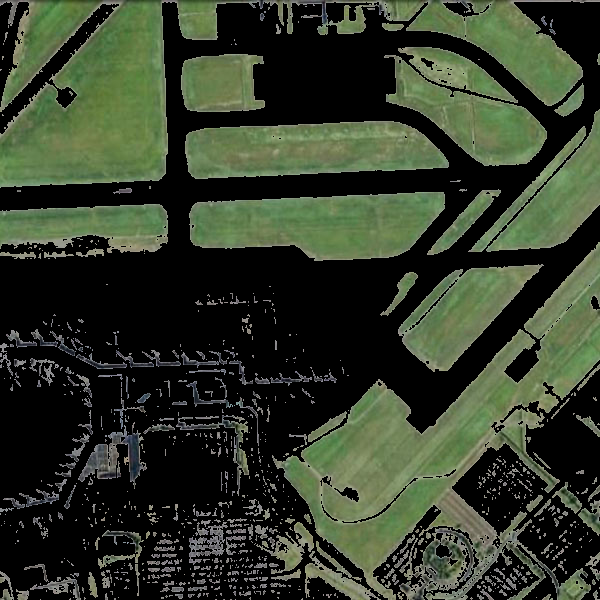
\includegraphics[width=\linewidth]{figure/airport_44_Class_01_Separated.png}
		\caption{分类一在原图片上的内容}
		\label{fig:airport_44_class_1_separated}
	\end{minipage}
	\begin{minipage}{0.45\linewidth}
		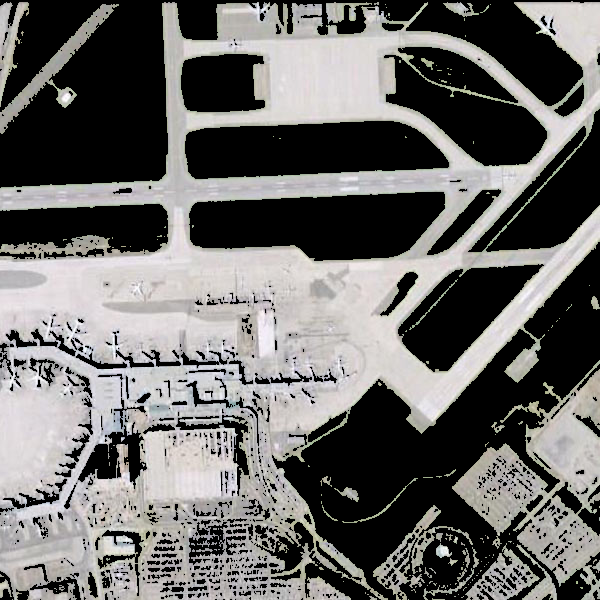
\includegraphics[width=\linewidth]{figure/airport_44_Class_02_Separated.png}
		\caption{分类二在原图片上的内容}
		\label{fig:airport_44_class_2_separated}
	\end{minipage}
\end{figure}
将k均值无监督分类过程进行统计分析,可以绘制如图\ref{fig:airport_44_animate}所示的图表\footnote{动画演示。如果不能播放可以尝试更换pdf阅读器,例如:Adobe Acrobat Reader。}。
\begin{figure}[H]
	\centering
	\animategraphics[autopause, autoresume, loop, autoplay, width=0.7\linewidth]{5}{figure/airport_44_Clustering_Latex_Animate/frame-}{0001}{0010}
	\caption{聚类点位置和分类过程(动画)}
	\label{fig:airport_44_animate}
\end{figure}
可以看到,在训练过程中,各像素点的分类会逐步收敛,最终达到稳定,形成最佳的分类结果。
	\section{实验五~监督分类}
	\subsection{实验目的}
\subsection{实验原理}
\begin{description}
	\item[监督分类的概念] 首先使用训练样本学习一个分类器,再对测试样本进行分类。
	\item[图像分类的两个步骤] 特征提取与分类算法。
	\item[特征提取] 颜色特征向量。
	\item[分类-训练过程] 使用训练样本学习分类器。
	\item[分类-测试过程] 使用学习好的分类器对测试样本分类。
\end{description}
\subsubsection{线性判别函数的定义}
直接用来对模式进行分类的准则函数。

若分属于$\omega_1$,$\omega_2$的两类模式可用一方程$d(\mathbf{X})=0$来划分,那么称$d(\mathbf{X})$为判别函数,或称判决函数、决策函数。
\begin{figure}[H]
	\centering
	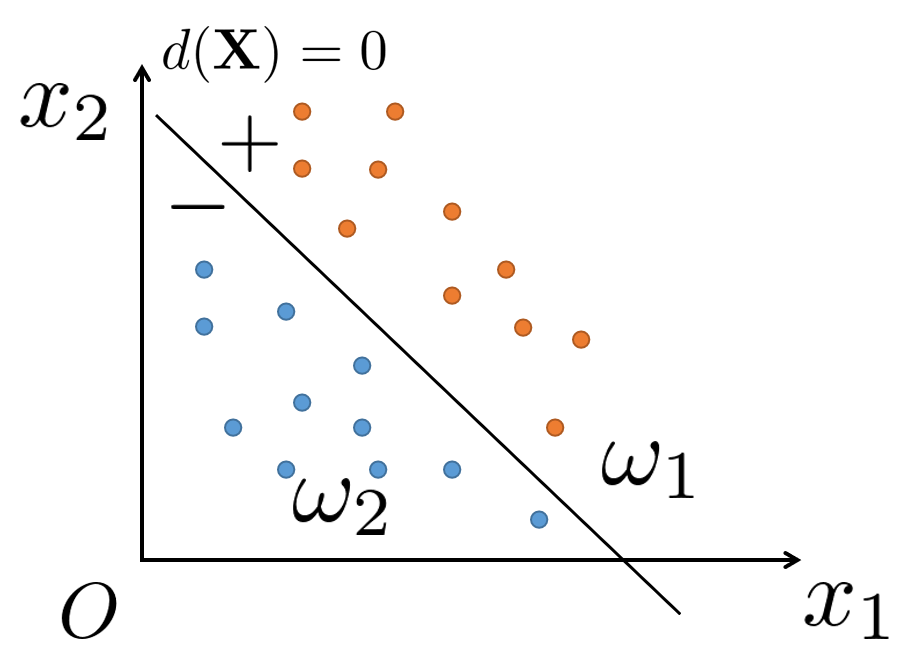
\includegraphics[width=0.7\linewidth]{figure/exp5classification}
	\caption{二类二维样本的分布}
	\label{fig:exp5classification}
\end{figure}
\begin{quote}
	\kaishu 例:一个二维的两类判别问题,模式分布如图所示,这些分属于$\omega_1$,$\omega_2$两类的模式可用一直线方程$d(\mathbf{X})=0$来划分。
	\[ d(\mathbf{X})=w_1x_1+w_2x_2+w_3=0 \]
	式中:$x_1$,$x_2$为坐标变量,$w_1$,$w_2$,$w_3$为方程参数。
\end{quote}
\subsubsection{多类情况}
\begin{description}
	\item[$\omega_i/\bar{\omega_i}$两分法] 用线性判别函数将属于$\omega_i$类的模式与其余不属于$\omega_i$类的模式分开。
\end{description}
\[ d_i(\mathbf{X})=\mathbf{W}_i^\mathsf{T}\mathbf{X}\begin{cases}
>0,\quad& \mathbf{X}\in\omega_i \\
<0,\quad& \mathbf{X}\in\bar{\omega_i}
\end{cases} \quad i=1,2,\dots,M \]
识别分类时:将某个待分类模式$\mathbf{X}$分别带入$M$个类的$d(\mathbf{X})$中,若只有$d(\mathbf{X})>0$,其他$d(\mathbf{X})$均$<0$,则判为$\omega_1$类。

对样本进行规范化处理,即$\omega_2$类样本全部诚意$(-1)$,则有
\[ d(\mathbf{X})=\mathbf{W}^\mathsf{T}\mathbf{X}>0 \]
感知器算法通过对已知类别的训练样本集的学习,寻找一个满足上式的权向量。

感知机算法步骤:
\begin{enumerate}
	\item 选择$N$个分属于$\omega_1$和$\omega_2$类的模式样本构成训练样本集
	\[ \left\lbrace \mathbf{X}_1,\mathbf{X}_2,\dots,\mathbf{X}_N \right\rbrace \]
	构成增广向量形式,并进行行规范化处理。任取权向量初始值$\mathbf{W}(1)$,开始迭代,迭代次数$k=1$。
	\item 用全部训练样本进行一轮迭代,计算$\mathbf{W}^\mathsf{T}(k)\mathbf{X}_i$的值,并修正权向量。分两种情况更新权向量的值:
	\begin{enumerate}
		\item 若$\mathbf{W}^\mathsf{T}(k)\mathbf{X}_i\leq 0$,分类器对第$i$个模式做了错误的分类。权向量矫正为:$\mathbf{W}(k+1)=\mathbf{W}(k)+c\mathbf{X}_i$($c$:正的矫正增量)。
		\item 若$\mathbf{W}^\mathsf{T}(k)\mathbf{X}_i> 0$,分类正确,权向量不变
		\[ \mathbf{W}(k+1)=\mathbf{W}(k) \]
	\end{enumerate}
	统一写为
	\[ \mathbf{W}(k+1)=\begin{cases}
	\mathbf{W}(k),\quad & \text{若}\mathbf{W}^\mathsf{T}(k)\mathbf{X}_i > 0 \\
	\mathbf{W}(k)+c\mathbf{X}_i, \quad & \text{若}\mathbf{W}^\mathsf{T}(k)\mathbf{X}_i \leq 0
	\end{cases} \]
	\item 分析分类结果:只要有一个错误分类,回到$2$,直至对所有样本正确分类。
\end{enumerate}
\subsection{实验流程}
\subsection{实验程序}
\subsection{实验结果和分析}
	\section{实验六~集成学习与分类性能评价}
	\subsection{实验目的}
理解集成学习的概念和评价分类器性能的评价方法,掌握一些典型的集成学习方法和分类器性能评价方法,例如Bagging方法。完成遥感图像的图像分类。
\subsection{实验原理}
\begin{description}
	\item[集成学习] 原理:构建并结合多个学习器来完成学习任务,提升泛化性能。
	\begin{figure}[H]
		\centering
		\begin{tikzpicture}[node distance=1.5cm]
		\node(classifier_1) [process] {个体学习器1};
		\node(classifier_2) [process, below of=classifier_1] {个体学习器2};
		\node(dots) [empty_process, below of=classifier_2] {$\vdots$};
		\node(classifier_3) [process, below of=dots] {个体学习器n};
		\node(combination) [process, right of=classifier_2, node distance=5cm] {结合模块};
		\node(output_classification) [io, right of=combination, node distance=5cm] {输出};
		
		\draw[arrow] (classifier_1) -- (combination);
		\draw[arrow] (classifier_2) -- (combination);
		\draw[arrow] (classifier_3) -- (combination);
		\draw[arrow] (combination) -- (output_classification);
		\end{tikzpicture}
	\end{figure}
	\item[个体学习器] 从训练数据学习的一个分类器,比如线性判别函数。个体学习器应好而不同。
	\item[Bagging方法] 思想:通过对训练数据集采样,得到不同的子集,每个子集训练一个个体学习器,使用相互交叠的子集。\\
	自助取样法:随机取出一个样本放入采样集,再把该样本放回初始数据集,使得下次采样时仍可能选中该样本。
	\item[集成学习——投票法] 对于一个数据进行分类,在不同学习器中可以会出现不同的分类结果。对于这种情况,这个数据最终的分类服从“少数服从多数”的原则,即采纳得到票数最高的分类判定。
\end{description}
\subsection{实验流程}
\begin{figure}[H]
	\centering
	\begin{tikzpicture}[node distance=1.5cm]
	\node(begin) [startstop] {开始};
	\node(input_img) [io, below of=begin] {读取待分类的图片};
	\node(abstracting_training_set) [process, below of=input_img] {提取训练样本};
	\node(generate_negative_training_set) [process, below of=abstracting_training_set] {生成负样本集};
	\node(sample_training_set) [process, below of=generate_negative_training_set] {抽取产生多个学习器使用的训练样本};
	\node(training_classifiers) [process, below of=sample_training_set] {训练多个学习器};
	\node(voting) [process, below of=training_classifiers] {投票产生最终的分类结果};
	\node(calculating_accuracy) [process, below of=voting] {计算正确率};
	\node(output_classification) [io, below of=calculating_accuracy] {输出显示分类结果};
	\node(end) [startstop, below of=output_classification] {结束};
	
	\draw[arrow] (begin) -- (input_img);
	\draw[arrow] (input_img) -- (abstracting_training_set);
	\draw[arrow] (abstracting_training_set) -- (generate_negative_training_set);
	\draw[arrow] (generate_negative_training_set) -- (sample_training_set);
	\draw[arrow] (sample_training_set) -- (training_classifiers);
	\draw[arrow] (training_classifiers) -- (voting);
	\draw[arrow] (voting) -- (calculating_accuracy);
	\draw[arrow] (calculating_accuracy) -- (output_classification);
	\draw[arrow] (output_classification) -- (end);
	\end{tikzpicture}
\end{figure}
\subsection{实验程序}
\lstinputlisting[caption={集成学习和正确率分析}]{"../Executable Script/Exp 6/EnsembleLearning.m"}
\lstinputlisting[caption={绘制矩形函数}]{"../Function Library/DrawRectangle.m"}
\lstinputlisting[caption={LDA分类器训练函数}]{"../Function Library/LDAClassification.m"}
\lstinputlisting[caption={LDA分类器生成分类逻辑函数}]{"../Function Library/LDAClassificationLogicMap.m"}
\lstinputlisting[caption={正确率计算函数}]{"../Function Library/ImageClassificationAccuracyJudgement.m"}
\subsection{实验结果和分析}
选择如图\ref{fig:airport_44_samples}所示的两块区域的数据作为训练样本,对学习器进行训练。
\begin{figure}[H]
	\centering
	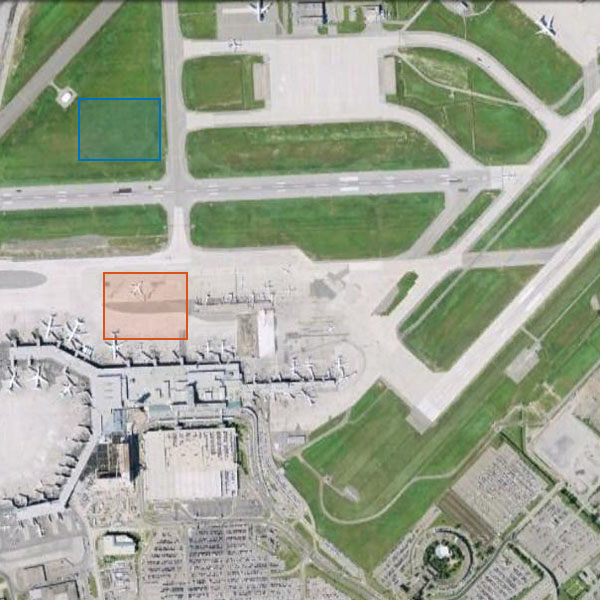
\includegraphics[width=0.7\linewidth]{figure/airport_44_Ensemble_Learning_Training_Set.png}
	\caption{训练样本的选取}
	\label{fig:airport_44_samples}
\end{figure}
对三个学习器进行训练,最终可以得到如下图所示的分类结果(白色区域代表该区域属于这个分类)。
\begin{figure}[H]
	\centering
	\begin{minipage}{0.45\linewidth}
		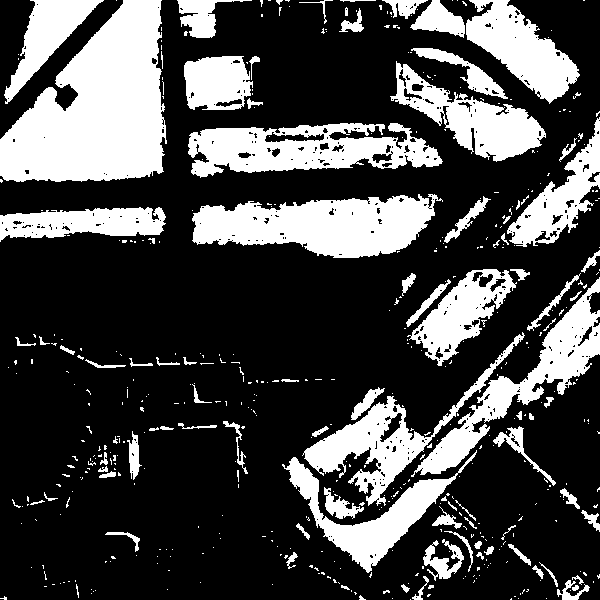
\includegraphics[width=\linewidth]{figure/airport_44_Classifier_1_Class_1.png}
		\caption{学习器1对分类1的分类结果}
	\end{minipage}
	\begin{minipage}{0.45\linewidth}
		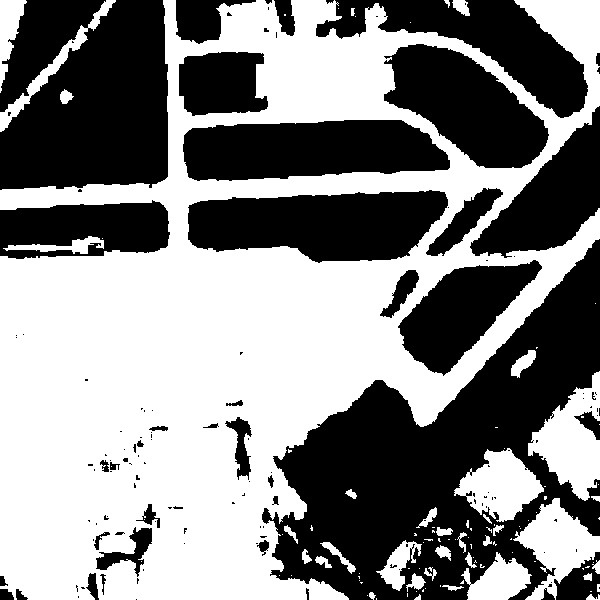
\includegraphics[width=\linewidth]{figure/airport_44_Classifier_1_Class_2.png}
		\caption{学习器1对分类2的分类结果}
	\end{minipage} \\
	\begin{minipage}{0.45\linewidth}
		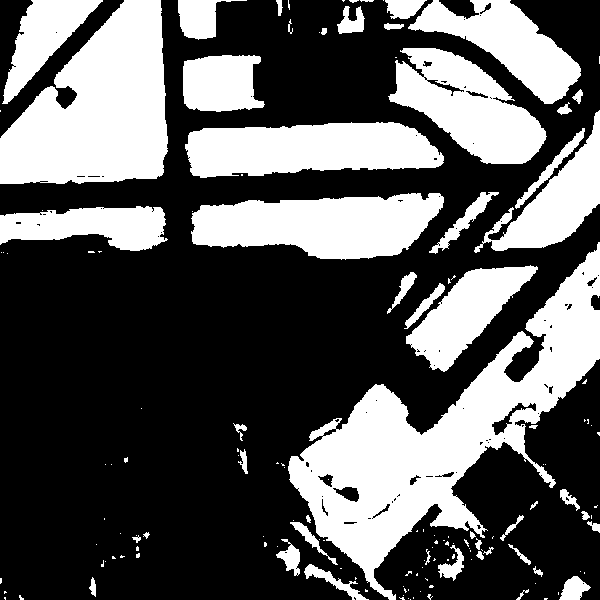
\includegraphics[width=\linewidth]{figure/airport_44_Classifier_2_Class_1.png}
		\caption{学习器2对分类1的分类结果}
	\end{minipage}
	\begin{minipage}{0.45\linewidth}
		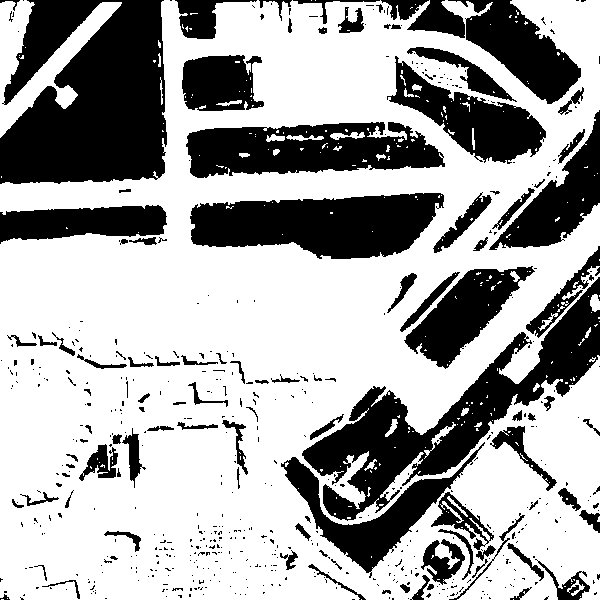
\includegraphics[width=\linewidth]{figure/airport_44_Classifier_2_Class_2.png}
		\caption{学习器2对分类2的分类结果}
	\end{minipage} \\
	\begin{minipage}{0.45\linewidth}
		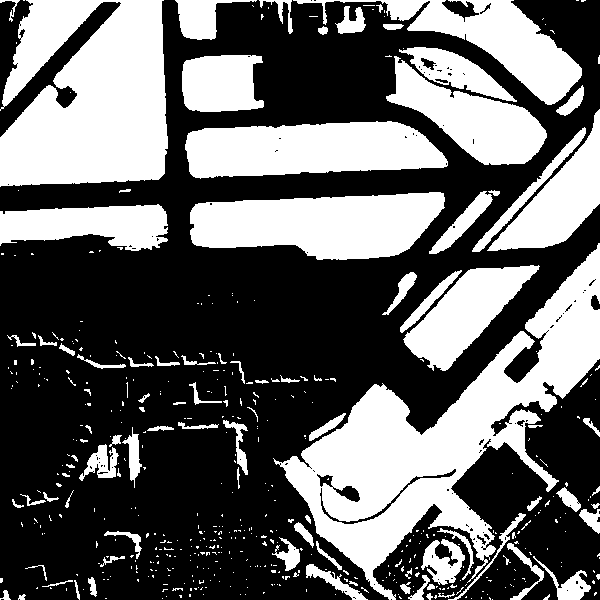
\includegraphics[width=\linewidth]{figure/airport_44_Classifier_3_Class_1.png}
		\caption{学习器3对分类1的分类结果}
	\end{minipage}
	\begin{minipage}{0.45\linewidth}
		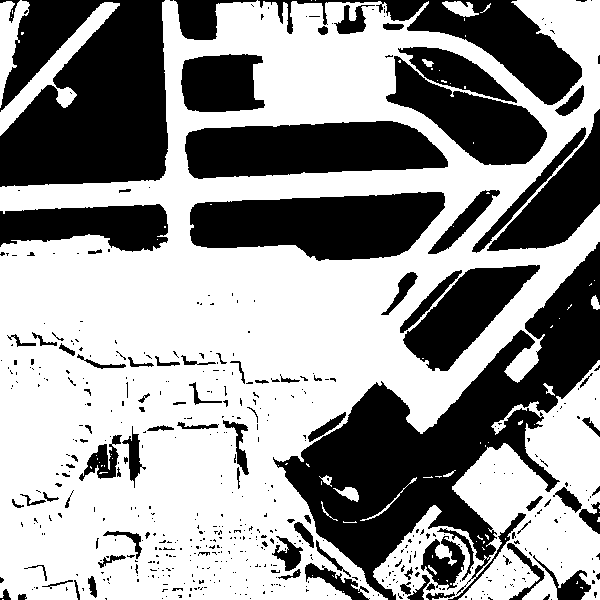
\includegraphics[width=\linewidth]{figure/airport_44_Classifier_3_Class_2.png}
		\caption{学习器3对分类2的分类结果}
	\end{minipage} 
\end{figure}
采用投票法对三个不同的学习器的分类结果进行合并,可以得到如下图所示的分类结果。
\begin{figure}[H]
	\centering	\begin{minipage}{0.45\linewidth}
		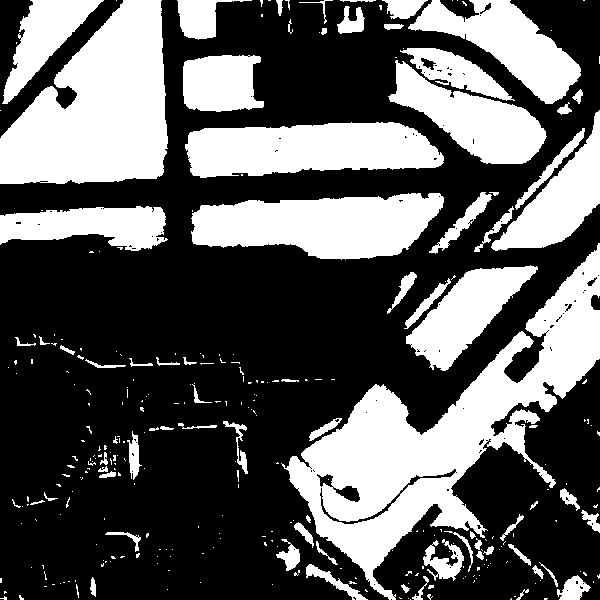
\includegraphics[width=\linewidth]{figure/airport_44_Class_1.png}
		\caption{分类1的分类结果}
	\end{minipage}
	\begin{minipage}{0.45\linewidth}
		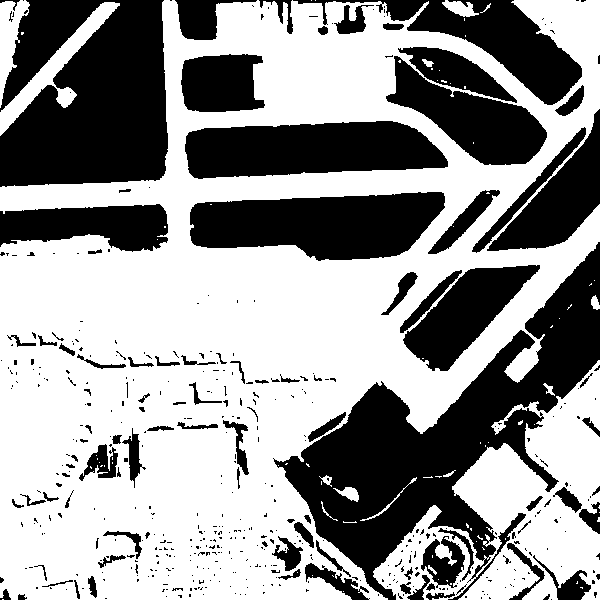
\includegraphics[width=\linewidth]{figure/airport_44_Class_2.png}
		\caption{分类2的分类结果}
	\end{minipage}
\end{figure}
对不同分类器的分类结果进行分析,可以得到它们的正确率,如下表所示。\\
\begin{tabular}{ccccc}
	\toprule
	算法 & 分类1 & 分类2 & 总正确率 & 平均正确率 \\
	\midrule
	分类器1 & 77.17\% & 86.45\% & 82.92\% & 82.92\% \\
	分类器2 & 97.40\% & 99.87\% & 98.93\% & 98.93\% \\
	分类器3 & 99.89\% & 99.71\% & 99.82\% & 99.82\% \\
	集成学习 & 97.32\% & 99.10\% & 98.84\% & 98.21\%  \\
	单个分类器 & 93.87\% & 94.20\% & 94.05\% & 94.04\% \\
	\bottomrule
\end{tabular}

从集成学习和分类的结果中分析,可以发现,由于线性判别函数的初始状态不同、训练样本不同,会导致最终的分类结果会有所不同,产生不确定性。而集成学习可以通过比较和处理来自不同分类器的分类结果,从而改善分类的效果,使分类的结果更加细致,减小不确定性。在多次尝试中,我发现选取的训练样本越多、分类器的数量越多,越能减小分类结果的不确定性,改善最终的分类结果,与此同时带来的代价就是要使用更多的计算资源和时间来对数据进行分类。
\end{document}